\documentclass[a4paper]{extarticle}
\usepackage[utf8]{inputenc}
\usepackage[a4paper, margin=1in]{geometry}

\usepackage{amssymb}
\usepackage{amsmath}
\usepackage{enumitem}
\usepackage{tcolorbox}
\usepackage{fancyhdr}
\usepackage{graphicx}
\usepackage{float}

\setlength{\parindent}{0em}
\setlength{\parskip}{0.4em}

\definecolor{theoremblue}{RGB}{1, 73, 124}
\definecolor{corollaryblue}{RGB}{70, 143, 175}
\definecolor{exampleblue}{RGB}{137, 194, 217}

\newtcolorbox{tbox}{colback=theoremblue!20,colframe=theoremblue,
boxrule=0pt,arc=0pt,boxsep=2pt,left=2pt,right=2pt,leftrule=2pt}

\newtcolorbox{cbox}{colback=corollaryblue!20,colframe=corollaryblue,
boxrule=0pt,arc=0pt,boxsep=2pt,left=2pt,right=2pt,leftrule=2pt}

\newtcolorbox{ebox}{colback=exampleblue!20,colframe=exampleblue,
boxrule=0pt,arc=0pt,boxsep=2pt,left=2pt,right=2pt,leftrule=2pt}

\title{FMFP - Lecture Notes Week 1}
\author{Ruben Schenk, ruben.schenk@inf.ethz.ch}
\date{\today}

\pagestyle{fancy}
\fancyhf{}
\rhead{ruben.schenk@inf.ethz.ch}
\rfoot{Page \thepage}
\lhead{FMFP - Lecture Notes Week 1}

\begin{document}

\maketitle
\newpage


\section{Introduction \& Basic Haskell Syntax}

\subsection{Example: GCD}

The \textbf{GCD problem} is given as follows: Compute the greatest common divisor of two natural numbers. We have the following \textit{specifications:} Let \(x, \, y \in \mathcal{N}\) be given. The number \(z\) is the \textbf{greatest common divisor} of \(x\) and \(y\) iff. \(z \, \mid \, x\) and \(z \, \mid \, y\) and there is no \(z'\), with \(z' > z\), such that \(z' \, \mid \, x\) and \(z' \, \mid \, y\). Here, \(z \, \mid \, x \equiv \exists a \in \mathcal{N}.a \cdot z = x\).

The problem specification is not \textbf{constructive,} i.e. it does not describe how the GCD should be computed.


\subsubsection{Imperative GCD}

\begin{verbatim}
    public static int gcd(int x, int y) {
        while(x != y) {
            if(x > y) {
                x = x - y;
            } else {
                y = y - x;
            }
        }
        return x;
    }
\end{verbatim}

The \textbf{imperative GCD}, as shown above, consists of control flow statements and assignments. Assignments change the computer's \textit{state.} To understand \verb|gcd|, one must understand how its state changes.

Poor man's reasoning would be to simulate and track the memory content during execution. A better way would be to use \textit{Hoare logic} in the form of \(\{P\} \text{ prog } \{Q\}\). Formal reasoning is possible, but not easy!

\subsubsection{Functional GCD}

\begin{verbatim}
    gcd x y
        | x == y    = x
        | x > y     = gcd (x - y) y
        | otherwise = gcd x       (y - x)
\end{verbatim}

The functional way formalizes \textit{what} should be computed, rather than \textit{how.} This is an algorithm, provided we have also specified how functions are executed.

\subsection{Basic Concepts in Functional Programming}

\subsubsection{Referential Transparency}

Functions compute values. But functions also \textit{are} values: we can compute and return them. It is important to note that functions in functional programming have \textbf{no side effects:} \verb|f(x)| always returns the same value. This in contrast to other programming languages we've known so far. Consider the following \verb|Java| example:

\begin{verbatim}
    class Test {
        static int y = 0;
        static int f(int x) {
            y = y + 1;
            return y;
        }
    }

    public static void main(String[] args) {
        System.out.println(f(0));
        System.out.println(f(0));
    }
\end{verbatim}

One will immediately see that this prints out \verb|0| and then \verb|1|, which means that \verb|f(0)| returns different values with the same input.

Since functions have no side effects, we can reason with the more easily in mathematics. This property is also called \textbf{referential transparency:} an expression evaluates to the same value in every context.

\subsubsection{Evaluation}

An \textbf{evaluation strategy} defines how and when expressions are evaluated during the execution of a program. We differ between two strategies:

\begin{itemize}
    \item \textit{Eager evaluation:} evaluate arguments first. Also called "call-by-value", corresponds to the left (green) path in the figure below.
    \item \textit{Lazy evaluation:} evaluate arguments only when needed (used by Haskell). Also called "call-by-need" (or "left-most/outermost"), corresponds to the right (blue) path in the figure below.
\end{itemize}

\begin{figure}[H]
    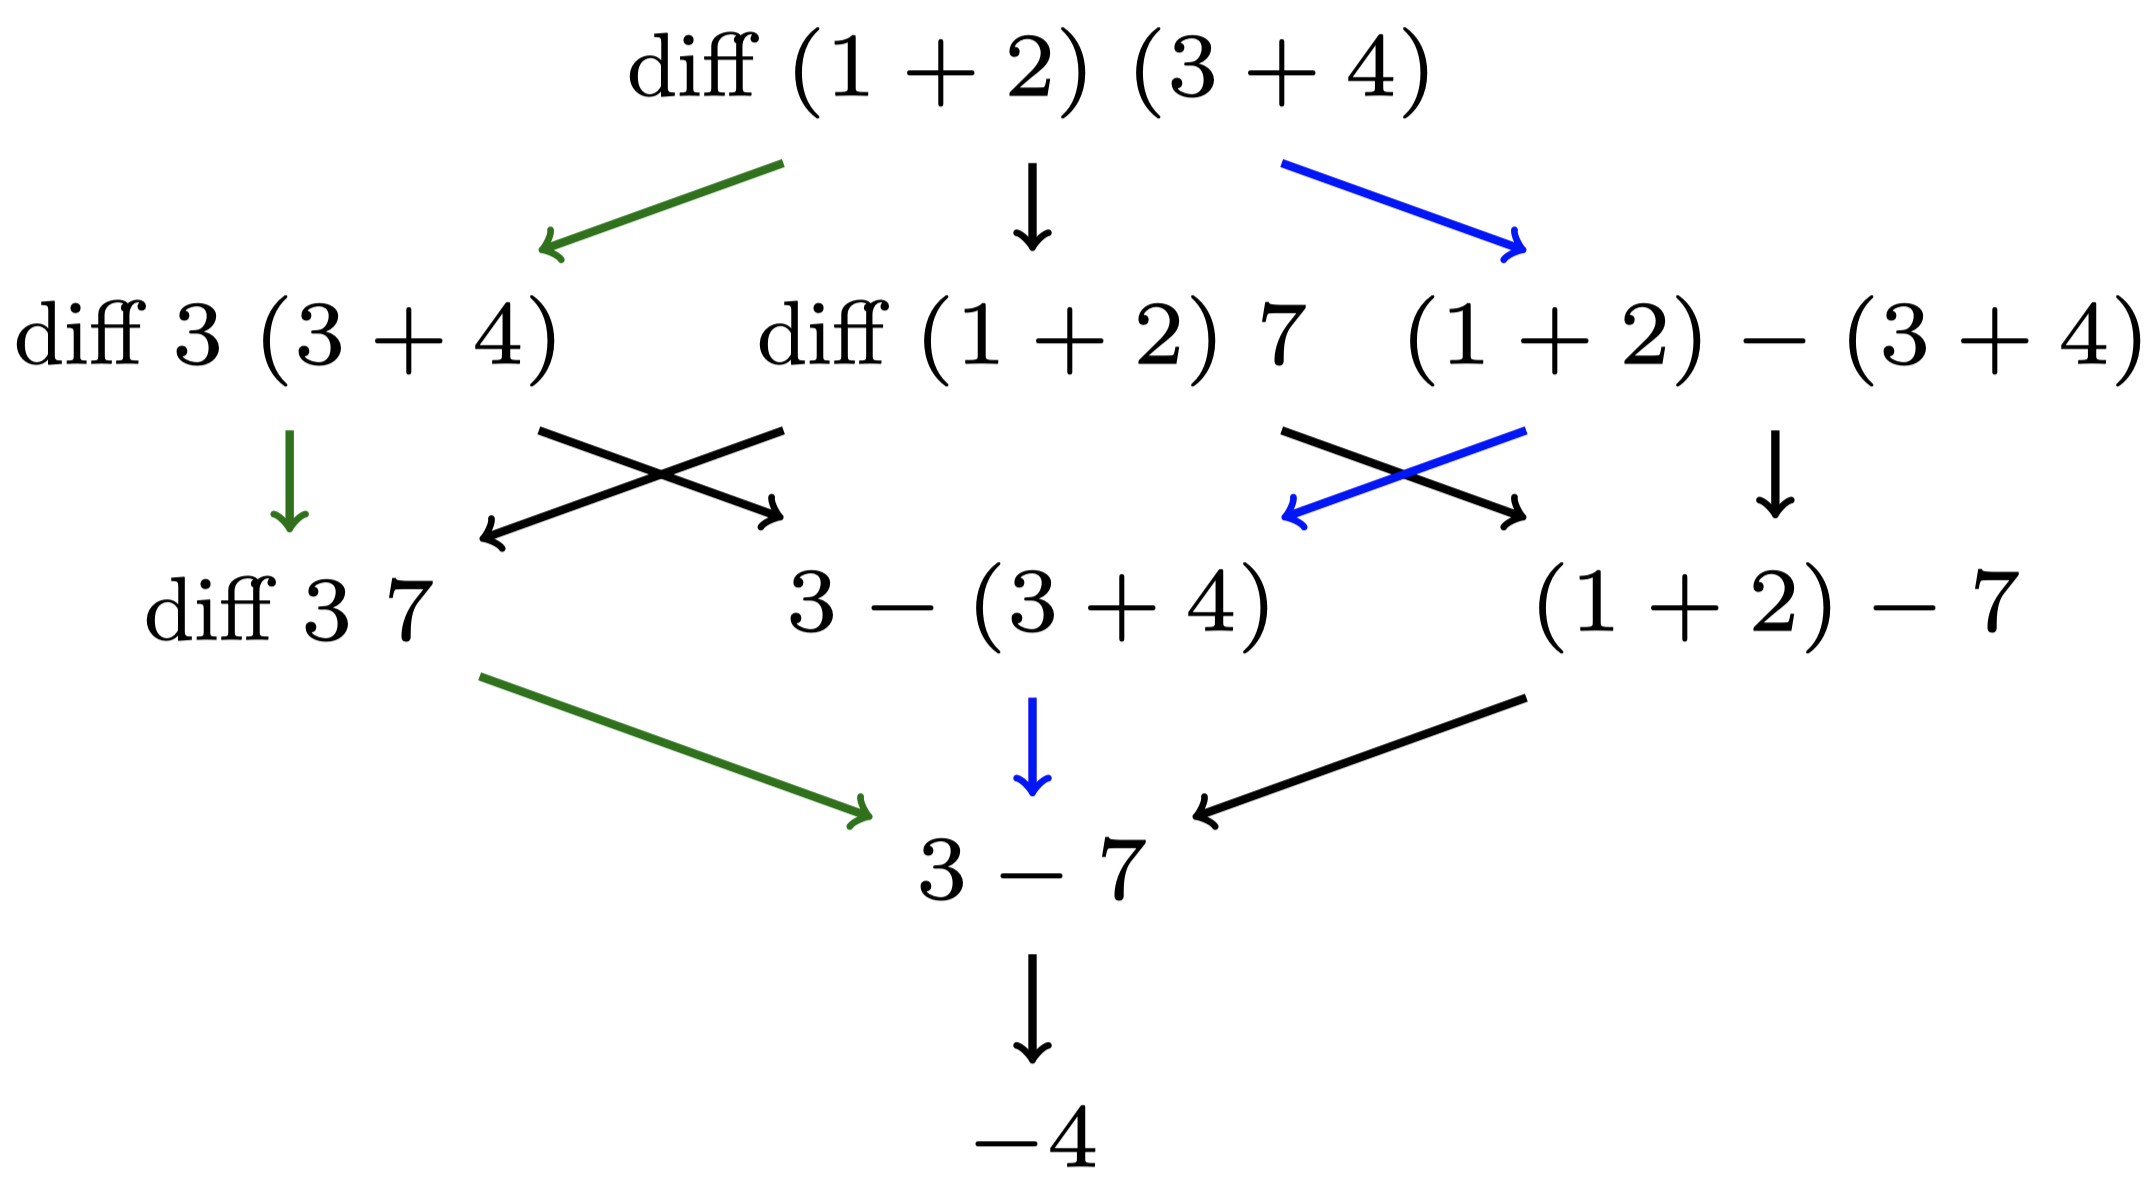
\includegraphics[width=10cm]{../images/FMFP_Fig1-1}
    \centering
\end{figure}

\subsection{Basic Haskell Syntax}

\subsubsection{Syntax and Types}

We present the basic syntax principles in the following code example:

\begin{verbatim}
    gcd x y        -- functions and arguments start with lower-case letters
        | x == y    = x
        | x > y     = gcd (x - y) y          -- arguments are written in sequence and
        | otherwise = gcd x       (y - x)    -- separated by whitespace
\end{verbatim}

Furthermore, functions consist of different cases and a program consists of several definitions:

\begin{verbatim}
    myConstant = 5

    afunction y1 y2 ... ym
        | guard1 = expr1
        | guard2 = expr2
        ...
        | guardm = exprm

    anotherFucntion z1 z2 ... zk = ...
\end{verbatim}

\textbf{Indentation} determines the separation of definitions. All function definitions must start at the same indentation level. If a definition requires \(n > 1\) lines, we indent lines \(2\) to \(n\) further. This leads to the following \textit{recommended layout:}

\begin{verbatim}
    f1 x1 x2
        | a long guard which may go over
          a number of lines
            = a long expression that can also go over
              several lines
        | g2 = expr2
    
    f2 x1 x2 x3 = ...
\end{verbatim}

\subsubsection{Functions}

Functions live in a global scope. This means that a function can be called from any other. Example:

\begin{verbatim}
    f x y = ...
    g x = ... h ...
    h z = ... f ... g ...
\end{verbatim}

We can define functions and variables in local scope with \verb|let| and \verb|where|:

\begin{verbatim}
    let x1 = e1
        ...
        xn = en
    in e
\end{verbatim}

\section{Natural Deduction}

\subsection{Introduction to Natural Deduction}

\subsubsection{Abstract Example (without Assumptions)}

Consider the following "meaningless" language:

\[
    \mathcal{L} = \{\oplus, \, \otimes, \, \times, \, +\}
\]

We furthermore state the following \textit{rules:}

\begin{itemize}
    \item \(\alpha\): If \(+\), then \(\otimes\)
    \item \(\beta\): If \(+\), then \(\times\)
    \item \(\gamma\): If \(\otimes\) and \(\times\), then \(\oplus\)
    \item \(\delta\): \(+\) holds
\end{itemize}

Our goal is to prove \(\oplus\). We might proceed as follows:

\begin{enumerate}
    \item \(+\) holds by \(\gamma\).
    \item \(\otimes\) holds by \(\alpha\) with \(1\).
    \item \(\times\) holds by \(\beta\) with \(1\).
    \item \(\oplus\) holds by \(\gamma\) with \(2\) and \(3\).
\end{enumerate}

We might also present this proof as a \textbf{derivation tree:}

\begin{figure}[H]
    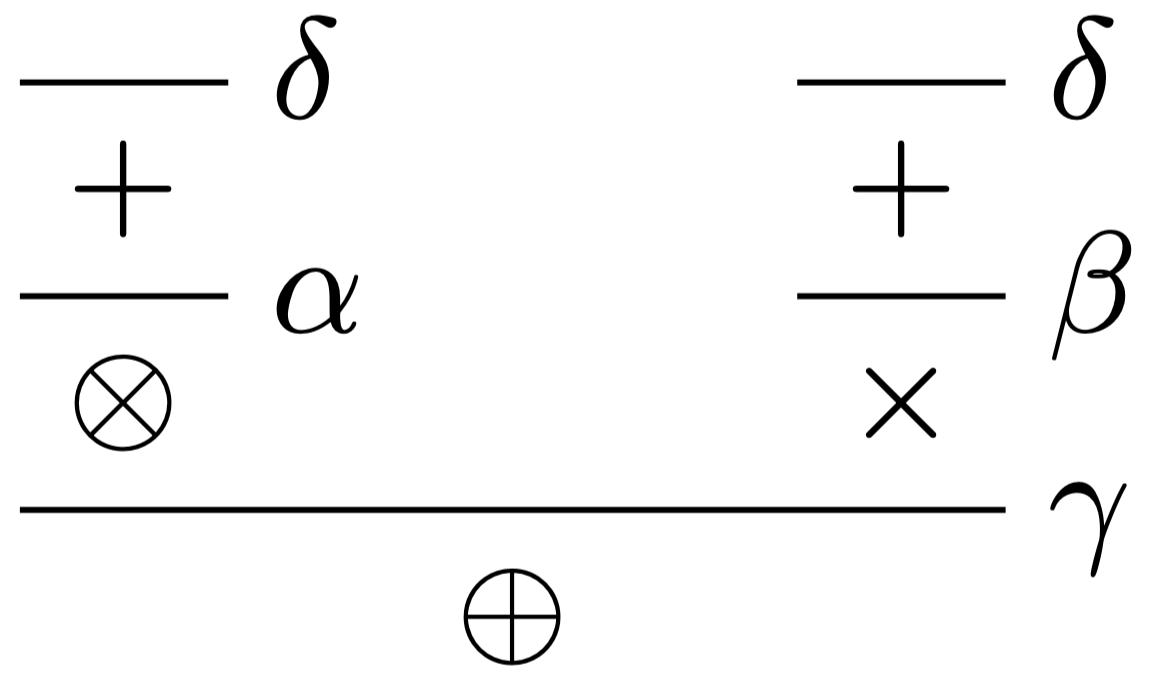
\includegraphics[width=6cm]{../images/FMFP_Fig1-2}
    \centering
\end{figure}

\subsubsection{Abstract Example (with Assumptions)}

We revisit the previous example by slightly changing one of our rules:

\begin{itemize}
    \item \(\alpha\): If \(+\), then \(\otimes\)
    \item \(\beta\): If \(+\), then \(\times\)
    \item \(\gamma\): If \(\otimes\) and \(\times\), then \(\oplus\)
    \item \(\delta\): We may assume \(+\) when proving \(\oplus\)
\end{itemize}

We can build the following proof system. In this system, \(\Gamma\) is the set of assumptions we make during our proof:

\begin{figure}[H]
    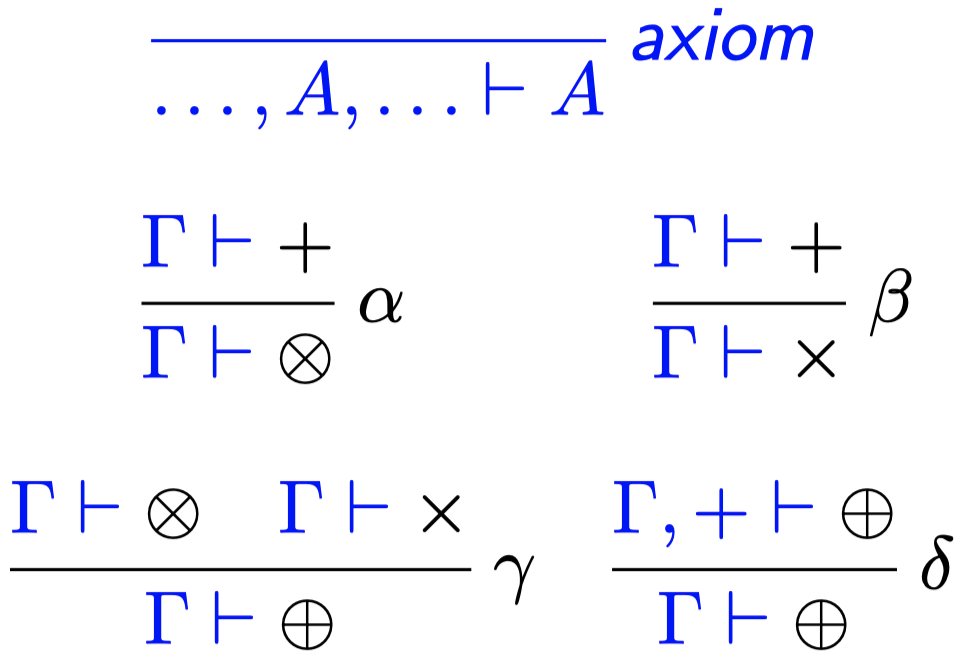
\includegraphics[width=6cm]{../images/FMFP_Fig1-3}
    \centering
\end{figure}

Our derivation tree from previously changes slightly to the following:

\begin{figure}[H]
    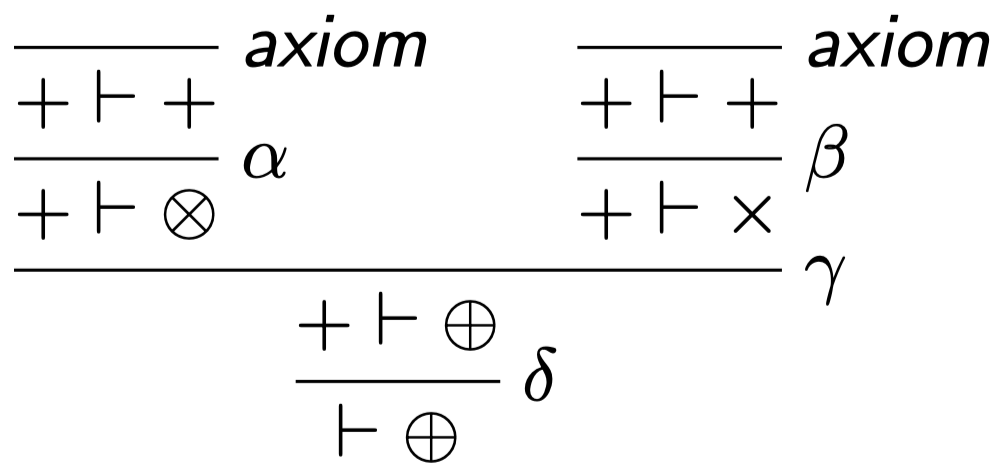
\includegraphics[width=6cm]{../images/FMFP_Fig1-4}
    \centering
\end{figure}

\subsubsection{Summary}

\textbf{Rules} are used to construct derivations under assumptions. \(A_1,...,A_n \vdash A\) reads as "\(A\) follows from \(A_1,...,A_n\)".

\textbf{Derivations} are trees as shown in the examples above.

A \textbf{proof} is a derivation whose root has no assumptions.

\subsection{Propositional Logic}

\subsubsection{Syntax}

\textbf{Propositions} are built from a collection of variables and closed under disjunction, conjunction, implication, etc. More formally, let a set \(\mathcal{V}\) of variables be given. \(\mathcal{L}_P\), the \textbf{language of propositional logic,} is the smallest set where:

\begin{itemize}
    \item \(X \in \mathcal{L}_P \text{ if } X \in \mathcal{V}\)
    \item \(\bot \in \mathcal{L}_P\)
    \item \(A \land B \in \mathcal{L}_P \text{ if } A \in \mathcal{L}_P \text{ and } B \in \mathcal{L}_P\)
    \item \(A \lor B \in \mathcal{L}_P \text{ if } A \in \mathcal{L}_P \text{ and } B \in \mathcal{L}_P\)
    \item \(A \to B \in \mathcal{L}_P \text{ if } A \in \mathcal{L}_P \text{ and } B \in \mathcal{L}_P\)
\end{itemize}

In the following: \(X\) ranges over variables, \(A\) and \(B\) over formulae.

\subsubsection{Semantics}

A \textbf{valuation} \(\sigma : \mathcal{V} \to \{\text{True, False}\}\) is a function mapping variables to truth values. Valuations are simple kinds of models (or interpretations). We denote the set of valuations as \(\text{Valuations}\).

\textbf{Satisfiability} is the smallest relation \(\vDash \subseteq \text{Valuations} \times \mathcal{L}_P\) such that:

\begin{itemize}
    \item \(\sigma \vDash X \text{ if } \sigma(X) = \text{True}\)
    \item \(\sigma \vDash A \land B \text{ if } \sigma \vDash A \text{ and } \sigma \vDash B\)
    \item \(\sigma \vDash A \lor B \text{ if } \sigma \vDash A \text{ or } \sigma \vDash B\)
    \item \(\sigma \vDash A \to B \text{ if whenever } \sigma \vDash A \text{ then } \sigma \vDash B\)
\end{itemize}

Note that \(\sigma \nvDash \bot\) for every \(\sigma \in \text{Valuations}\).

We furthermore introduce the following characteristics about propositional logic:

\begin{itemize}
    \item A formula \(A \in \mathcal{L}_P\) is \textbf{satisfiable} if \(\sigma \vDash A\), for some valuation \(\sigma\)
    \item A formula \(A \in \mathcal{L}_P\) is \textbf{valid} (a \textbf{tautology}) if \(\sigma \vDash A\), for all valuations \(\sigma\)
    \item \textbf{Semantic entailment:} \(A_1,...,A_n \vDash A\) if for all \(\sigma\), if \(\sigma \vDash A_1,..., \, \sigma \vDash A_n\) then \(\sigma \vDash A\)
\end{itemize}

\begin{ebox}
    \textbf{Examples:}

    \begin{itemize}
        \item \(X \land Y\) is satisfiable as \(\sigma \vDash X \land Y\) for \(\sigma(X) = \sigma(Y) = \text{True}\)
        \item \(X \to X\) is valid
        \item \(\lnot  X, \, X \lor Y \vDash Y\) holds as \(\sigma \vDash \lnot X\) and \(\sigma \vDash X \lor Y\) constraint \(\sigma\) to \(\sigma(X) = \text{False}\) and \(\sigma(Y) = \text{True}\), so \(\sigma \vDash Y\)
    \end{itemize}
\end{ebox}

\subsubsection{Requirements}

We need some \textbf{requirements} for \textit{deductive systems.} The main requirement is that syntactic entailment \(\vdash\) (derivation rules) and semantic entailment \(vDash\) (truth tables) should agree. This requirement has two parts:

\begin{itemize}
    \item \textbf{Soundness:} If \(\Gamma \vdash A\) can be derived, then \(\Gamma \vDash A\).
    \item \textbf{Completeness:} If \(\Gamma \vDash A\), then \(\Gamma \vdash A\) can be derived.
\end{itemize}

Here, \(\Gamma \equiv A_1,...,A_n\) is some collection of formulae.

\subsubsection{Natural Deduction for Propositional Logic}

A \textbf{sequent} is an assertion (judgement) of the form \(A_1,...,A_n \vdash A\), where all \(A,A_1,...,A_n\) are propositional formulae. A \textbf{proof} of \(A\) is a derivation tree with root \(\vdash A\). If the deductive system is sound, then \(A\) is a tautology.

\paragraph{Conjunction}

\textbf{Conjunction} proposes rules of two kinds: \textit{introduce} and \textit{eliminate} connectives. The rules are given as follows:

\begin{figure}[H]
    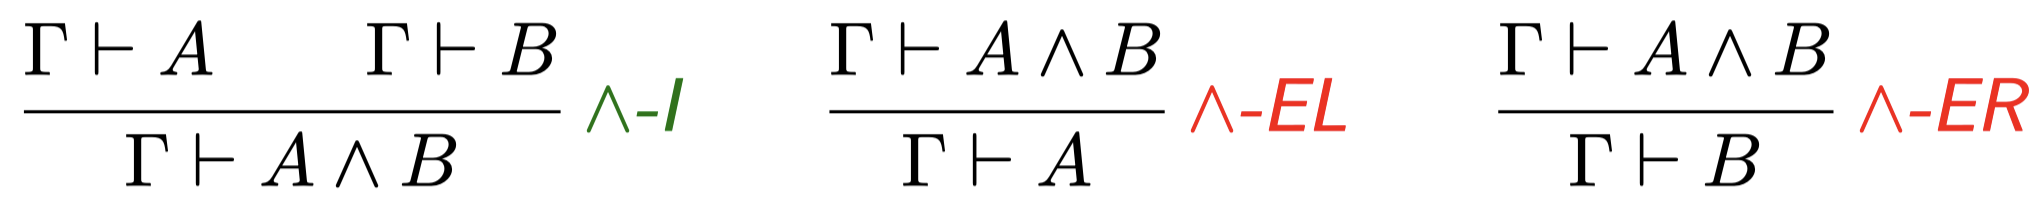
\includegraphics[width=10cm]{../images/FMFP_Fig1-5}
    \centering
\end{figure}

\begin{ebox}
    \textbf{Example:} The following figure shows an example derivation using conjunction rules.

    \begin{figure}[H]
        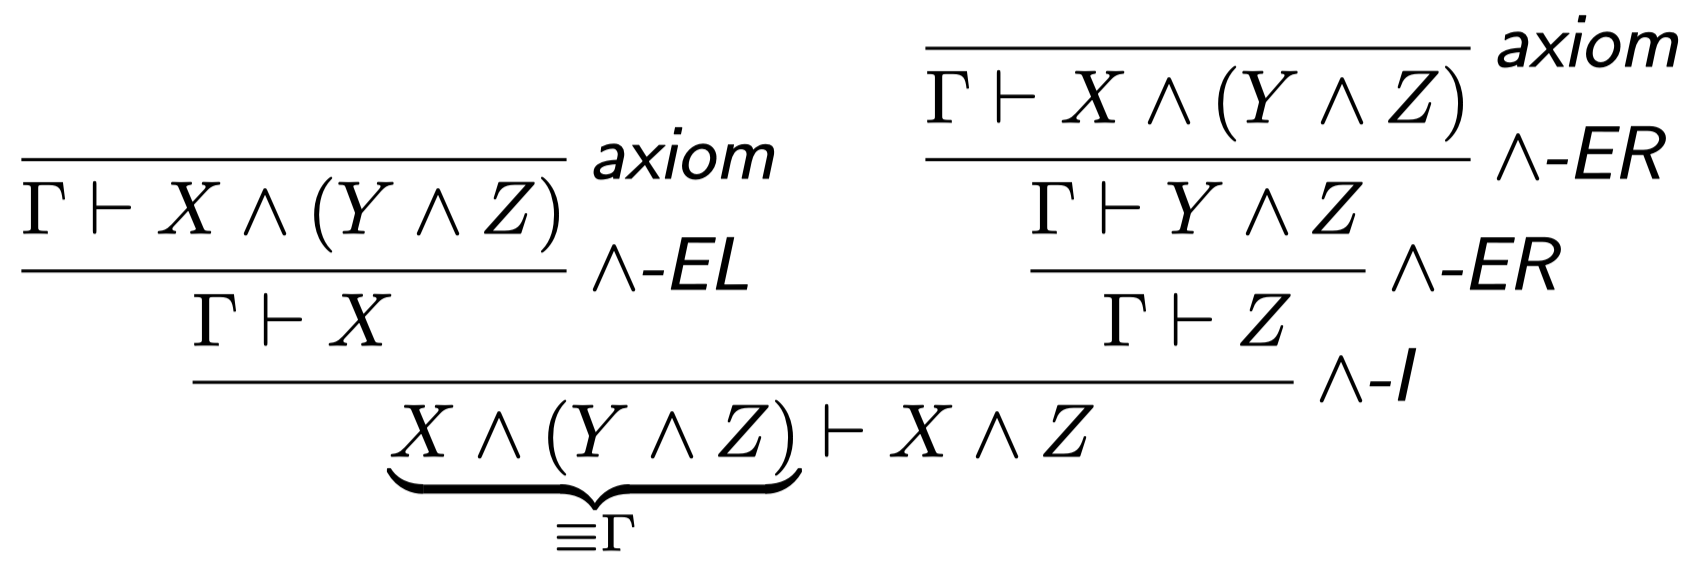
\includegraphics[width=10cm]{../images/FMFP_Fig1-6}
        \centering
    \end{figure}
\end{ebox}

\paragraph{Implication}

The rules for \textbf{implication} are given as follows:

\begin{figure}[H]
    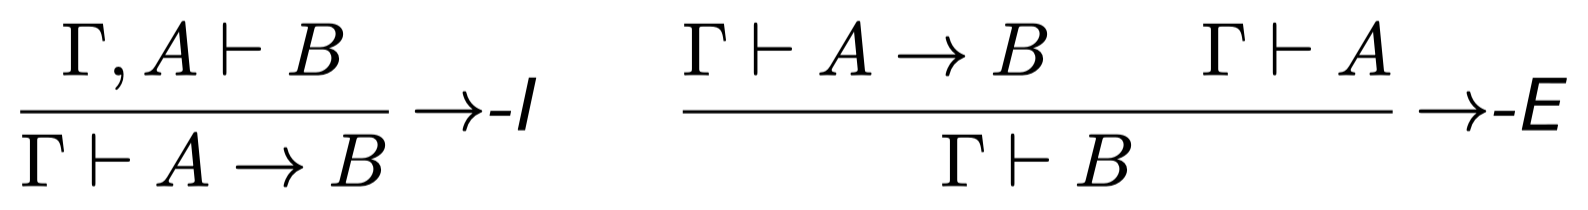
\includegraphics[width=8cm]{../images/FMFP_Fig1-7}
    \centering
\end{figure}

\paragraph{Disjunction}

The rules for \textbf{disjunction} are given as follows:

\begin{figure}[H]
    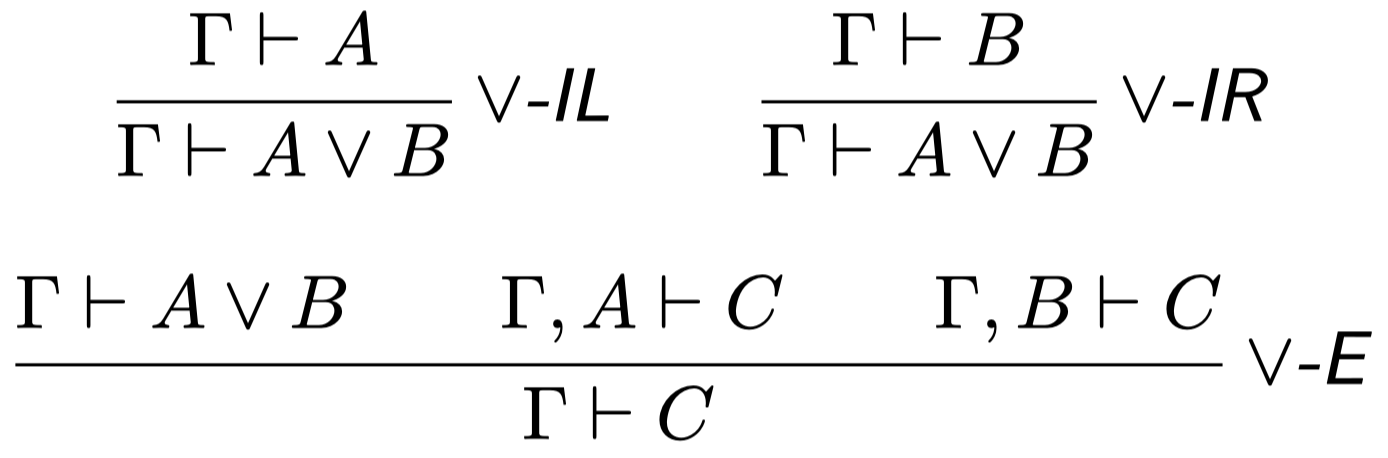
\includegraphics[width=7cm]{../images/FMFP_Fig1-8}
    \centering
\end{figure}

\end{document}